\documentclass[xcolor=dvipsnames,split]{beamer}
% bibstuffs:
\usepackage[sort&compress]{natbib}
\bibliographystyle{apsr}
\bibpunct[:]{(}{)}{;}{a}{,}{,}

%\usepackage[all]{xy}
%\input xy
%\xyoption {all}

\usepackage{beamerthemesplit}
\usecolortheme[rgb={0,0,.611764706}]{structure}
\definecolor{DukeBlue}{rgb}{0,0,.611764706}
\usetheme[height=11mm]{Rochester}
\setbeamertemplate{items}[ball]
\usepackage{rotating,amssymb,subfigure,tabularx}
\usepackage{caption}
\usepackage{graphicx}
\usepackage{color}
\usepackage{multicol}
\usepackage{array}
\usepackage{dcolumn}
\usepackage{multirow}
\usepackage{caption}
\setbeamerfont{tablefont}{size=\tiny}
\setbeamerfont{quotefont}{size=\small}



%\usepackage[all]{xy}
%\input xy
%\xyoption {all}

%\usepackage{booktabs}

%\graphicspath{{APSA-WDC/graphics/}}

 


\author[J.M. Montgomery, F.M. Hollenbach, M.D. Ward] % (optional, use only with lots of authors)
{Jacob M. Montgomery  \inst{1} \and Florian M. Hollenbach  \inst{2} \and Michael D. Ward \inst{2}}
% - Give the names in the same order as the appear in the paper.
% - Use the \inst{?} command only if the authors have different
%   affiliation.

\institute[] % (optional, but mostly needed)
{
  \inst{1}%
Department of Political Science\\
Washington University in St. Louis
  \and
  \inst{2}%
  Department of Political Science\\
  Duke University}

 
\title[APSA, New Orleans, LA, August/September, 2012]{\textsc{Say Yes to the Guess: \\ Tailoring Elegant Ensembles on a Tight
  (Data) Budget}}


\date{\today}


\begin{document}


\frame{\titlepage}


\section{Introduction}

\frame{\frametitle{Ensemble Bayesian Model Averaging (EBMA)}
\only<1>{
EBMA is principled way of combining a number of different prediction models to increase out-of-sample predictive power
\begin{itemize}
\item Component models are weighted based on predictive performance in calibration period
\item The EBMA prediction is then a finite mixture model of the different component models
\item The predictive pdf for the EBMA model can be written as: $p(y|f_{1}^{t^\ast}, \ldots,
f_{K}^{t^\ast})=\overset{K}{\underset{k=1}{\sum}} w_k g_k(y|f_{k}^{t^*})$, where $w_k$ are the weights associated with each model
\end{itemize}
}

\only<2>{
\begin{itemize}
\item Model weights are estimated using an expectation-maximization (EM) algorithm
\item More accurate models in the calibration period receive higher weights
\item Models making more unique predictions are favored
\end{itemize}
}
}
\section{EBMA Adjustment}

\frame{\frametitle{Adjusting EBMA to Forecasting in the Social Sciences}     
\only<1>{
Forecasting efforts in the social sciences are often hampered by data problems
\begin{itemize}
\item Often observations are missing
\item Rarely are missing observations truly random
\item Numerous forecasting models, but few true data observations to calibrate
\end{itemize}
}

\only<2>{
\begin{itemize}
\item To incorporate models with missing data we adjust the EM algorithm following Fraley, Raftery and Gneiting (2010) 
\item To make small sample adjustments we introduce a ``wisdom of the crowds'' parameter $c \in [0,1]$ 
\item Thus when estimating model weights, for each model there is a minimum $\frac{c}{k}$ probability that the observation is best represented by this model 
\end{itemize}

%% I don't know how much math you want to have in these slides....
}
}

\section{Applications}

\frame{\frametitle{Applying EBMA to Predict Quarterly Unemployment in the US}     
\only<1>{
\begin{itemize}
\item Predictions from the Survey of Professional Forecasters (SPF) from the Philadelphia Federal Reserve Bank
\item Green Book of the Fed
\item Predictions four quarters into the future
\item Rolling calibration window of ten quarters
\item Minimum of five forecasts in the calibration period for model inclusion
\end{itemize}
}

\only<2>{
\begin{figure}[h]
\caption{Observed and forecasted U.S. unemployment (1981-2007)}
\label{timeSeries}
\begin{center}
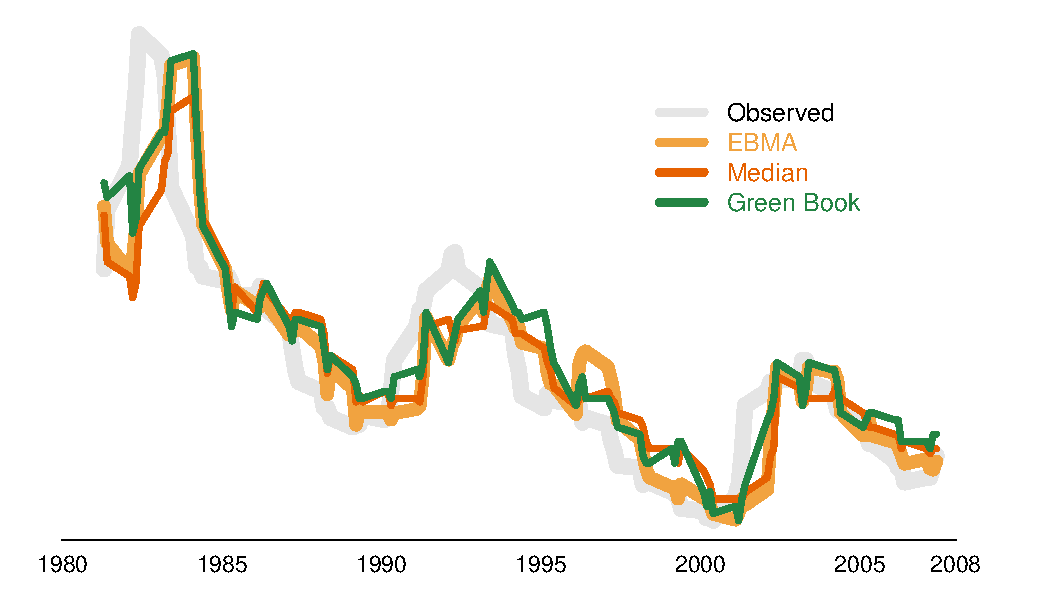
\includegraphics[scale=.6]{mdwtimeSeries2}
\end{center}
\end{figure}
}

\only<3>{
\begin{table}[h]
%\caption{Comparing adjusted EBMA models with Green Book, median, and mean forecasts of U.S. Unemployment (1981-2007)}
%\begin{center}
\begin{tiny}
\begin{tabular}{lrrrrrrrr}
\hline
 & MAE & RMSE & MAD & RMSLE & MAPE & MEAPE & MRAE & PW \\ 
\hline
 EBMA (c=0)& 0.54 & 0.74 & 0.37 & 0.093 & 8.37 & 6.49 & \textbf{0.73} & \textbf{27.36} \\ 
  EBMA (c=0.05)& \textbf{0.54} & 0.74 &\textbf{ 0.37} & \textbf{0.093} & \textbf{8.33} & \textbf{6.30} & 0.75 & \textbf{27.36} \\ 
 EBMA (c=0.1)& 0.54 & 0.74 & 0.35 & 0.093 & 8.40 & 6.44 & 0.76 & 28.30 \\ 
EBMA (c=1) & 0.61 & 0.80 & 0.46 & 0.102 & 9.72 & 8.92 & 0.95 & 46.23 \\ 
 Green Book& 0.57 & \textbf{0.73} & 0.43 & 0.093 & 9.37 & 8.81 & 1.00 & 45.28 \\ 
 Forecast Median& 0.62 & 0.81 & 0.47 & 0.103 & 9.83 & 8.87 & 0.98 & 47.17 \\ 
Forecast Mean& 0.61 & 0.80 & 0.46 & 0.102 & 9.71 & 9.06 & 0.93 & 46.23 \\ 
\hline
\end{tabular}
\end{tiny}
\end{table}
%\end{center}
}
}

\frame{\frametitle{Predicting the Incumbent Voteshare in the 2012 Presidential Election}     
\only<1>{
\begin{table}
\caption{Pre-election forecasts of the percent of the two-party vote going to the incumbent party in U.S. Presidential elections}
\begin{tiny}
\begin{tabular}{rlrrrrrrrrr}
  \hline
  & F & A & C & H & LBRT & L & Hol & EW & Cuz \\ 
  \hline
  1992 & 55.7 & 46.3 & 49.7 & 48.9 & 47.3 &  &  &  &  \\ 
  1996 & 49.5 & 57.0 & 55.5 & 53.5 & 53.3 &  & 57.2 & 55.6 &  \\ 
  2000 & 50.8 & 53.2 & 52.8 & 54.8 & 55.4 & 60.3 & 60.3 & 55.2 &  \\ 
  2004 & 57.5 & 53.7 & 52.8 & 53.2 & 49.9 & 57.6 & 55.8 & 52.9 & 51.1 \\ 
  2008 & 48.1 & 45.7 & 52.7 & 48.5 & 43.4 & 41.8 & 44.3 & 47.8 & 48.1 \\ 
\hline
\end{tabular}
\end{tiny}
\end{table}
}

\only<2>{
\begin{table}[ht]
\caption{Model weights and in-sample fit statistics for EBMA model of U.S. Presidential Elections (1992-2008)}
\label{presModel}
\begin{footnotesize}
\begin{center}
\begin{tabular}{lrrrr}
\hline
 & \shortstack{EBMA\\ Weight}&RMSE &MAE \\ 
\hline
EBMA &  & 1.92 & 1.56 \\ 
  Fair & 0.02 & 5.53 & 4.58 \\ 
  Abramowitz & 0.78 & 2.02 & 1.72 \\ 
  Campbell  & 0.07 & 3.46 & 2.88 \\ 
  Hibbs  & 0.04 & 2.68 & 2.44 \\ 
  Lewis-Beck, Rice, and Tien & 0.06 & 2.78 & 2.28 \\ 
  Lockerbie  & 0.00 & 7.33 & 6.97 \\ 
 Holbrook & 0.01 & 5.73 & 4.77 \\ 
  Erikson and Wlezien & 0.02 & 2.74 & 2.25 \\ 
  Cuz\`an & 0.00 & 1.27 & 0.95 \\ 
\hline
\end{tabular}
\end{center}
\end{footnotesize}
\end{table}
}

\only<3>{
\begin{figure}[h]
\caption{Predictive ensemble PDFs of incumbent-part vote share in U.S. Presidential Elections}
\label{pres}
\begin{center}
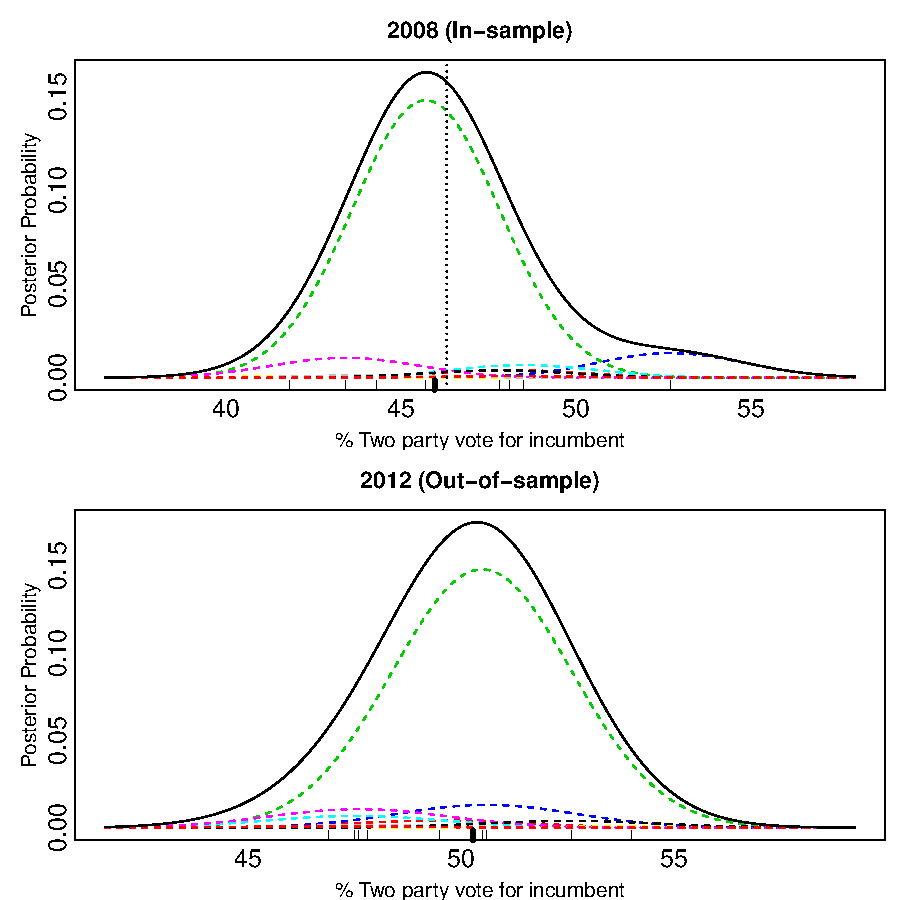
\includegraphics[scale=.3]{presForecast}%%% change this to only 2012
\end{center}
\end{figure}
}
}


\section{Conclusion}
\frame{\frametitle{Conclusion}     
\only<1>{
\begin{itemize}
\item d
\item d
\item d
\end{itemize}
}
}
\end{document}\bye

